\documentclass[12pt,a4paper]{article}
\usepackage{ctex}
\usepackage{graphicx}
\usepackage{appendix}
\usepackage{amsmath}
\usepackage{amsfonts}
\usepackage{hyperref}
\usepackage{fancyhdr}
\usepackage[left=3cm,right=3cm,top=2cm,bottom=2cm]{geometry}

\pagestyle{fancy}
\fancyhead[L]{\subsectionmark}
\renewcommand{\sectionmark}[1]{\markright{\thesection\ #1}} 
\fancyhf{}
\fancyhead[R]{\bfseries\thepage} 
\fancyhead[L]{\bfseries\rightmark} 
%\fancyhead[RE]{\bfseries\leftmark} 
\renewcommand{\headrulewidth}{0.4pt} 
\renewcommand{\footrulewidth}{0pt}


\title{数学分析的主线,高等数学的一切:\\连续函数与“有理”分析}
\author{BlackSmith\\ \& Typesetted by LoGanZhu}

\begin{document}
	{\bfseries\maketitle}\newpage
	{\large\tableofcontents}
	\newpage
	这里要讨论的,是关于{\bfseries 数学分析}(以及工科生的{\bfseries 高等数学})这门课程本身的某些中心思想和知识内容的组织方式。我并不是数学教师,甚至不是数学系学生,但是我作为一个“业余”读者,还是从这门课程中发现了一些自己以前没有注意过的东西。在此分享出来,供大家参考和批评。
	
	\section{连续函数的意义}{
		首先,让我们从一个高等数学中再熟悉不过的概念——{\bfseries 连续性}说起。所谓函数的连续性定义如下:
		\begin{quote} \itshape
			设实函数$f(x)$在点$x_0$及其附近有定义。若给定一任意小的$\varepsilon>0$,总能找到对应的$\delta>0$使得$\mid f(x)-f(x_0)\mid <\varepsilon$对所有的$\mid x-x_0\mid <\delta$都成立,则称$f(x)$在$x_0$处{\bfseries 连续}。若一个函数在其定义域内都连续,则常称该函数为{\bfseries 连续函数}。
		\end{quote}
	
		我在这里没有直接使用极限的记法,仍然用$\varepsilon-\delta$方法表述了一遍。“连续”两个字究竟是在说什么呢?如果我们直观地把定义翻译成自然语言,就是说:如果函数在其定义域内某一点(且称其为中心点)附近,总是可以划出一片足够小的区域,使得该区域内的函数值都与函数在中心点处的值充分接近,那么就称这个函数在该点处连续。归根结底,我们不如说:函数在某点连续,就是说函数在此足够平坦,足够光滑。这是我们能够从各种连续函数的图像所得到的一种印象。
		\begin{center}
			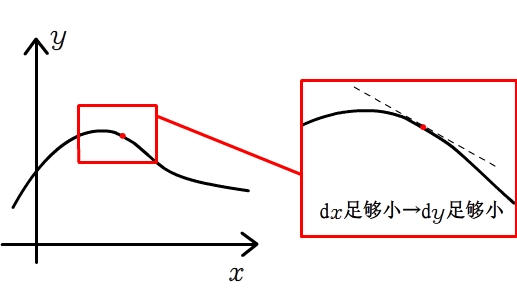
\includegraphics[width=12cm]{o.jpg}
		\end{center}
		我们可以说,连续性是一种{\itshape 较好}的性质,因为很多函数并不能满足连续性的要求。一些函数在若干个离散的点上不连续,这里引出了关于间断点的讨论;另一些函数则干脆是处处不连续,比如在教材中常常讨论的诸如Dirichlet函数与Riemann函数之类。尽管如此,这里却要给出对微积分课程给出一个关键的断语,那就是:
		\begin{quote} \itshape
			连续函数是数学分析课程(理科)的主线,更是高等数学课程(工科)所讨论的几乎全部内容。
		\end{quote}
		在已经指出许多常见常用但并不连续的函数之后,为何我们仍然会得到这样一个结论呢?我们不妨再回头看看连续函数究竟有怎样的特性。
		
		\subsection{连续函数类是实函数类的“杰出代表”}{
			关于连续函数,有一个很不起眼的命题——这个  命题\footnote{在实函数理论中有许多其他更加重要深刻、重要的结论,它们足以概括这个命题所叙述的有关特性(否则这个命题也该作为一条定理列入教材当中了)。我在本文中就这一命题大写特说的原因无非在于,它比那些重要结论更加通俗易懂,便于之后行文的展开与读者的理解接受。}  常常作为一些数学分析乃至实变函数教材课后一道简单的习题列出,而工科生则可能没有接触过这个命题。其内容大致是这样的:
			\begin{quote} \itshape
				{\bfseries 命题}:设有两函数$f_1(x)$,$f_2(x)$均在一开区间$(a,b)$上连续,其中$a<b$为两个任意的实数。若$f_1(x)$与$f_2(x)$在$(a,b)$内所有的有理点处取值相同,即
				\[\boldsymbol{f_1(x)=f_2(x)(\forall x<\mathbb{Q})}\]
				则函数$f_1(x)$,$f_2(x)$必然在$(a,b)$上所有点处都取值相同,即它们在区间上是同一个函数。
			\end{quote}
			
			这个命题换句话说,就是:对于一个连续函数而言,只需要其在某区间$(a,b)$上所有有理点上的值,就可以完全确定这个连续函数在$(a,b)$内的情况,尽管我们甚至还不知道这个函数在那比有理点“多得多”(这个所谓的“多”当然不是严格描述)的无理点上究竟为何值——事实上大多数情况下我们也无法算出。
			
			对于数学系的学生而言,这一命题看起来是十分普通的,至多不过为一道普通的练习题罢了;但是,如果我们现在是处在一个数学理论之“局外人”的视角来看待这个命题,我们不能不说这样一个结果是极其值得思考的。为了便于读者理解这个命题的深层内涵,这里我们还是有必要把这个命题证明一下,尽管所用的工具仍然是对于一般人而言显得枯燥无味的$\varepsilon−\delta$理论(也就是利用前面那条连续性的定义来证明)。
			
			\vspace{22pt}\hrule\vspace{11pt}
			{\bfseries 证明}:我们现在需要做的事情,就是证明满足题设的这样两$f_1(x)$,$f_2(x)$	在区间$(a,b)$上的所有无理点处也取相同的值。现在任取一个介于$a,b$之间的无理数$x_0$,那么我们要做的事情就是证明$f_1(x_0)=f_x(x_0)$的成立。考虑到这两个函数在无理点$x_1$处都是连续的,因而对于任给的$\varepsilon>0$,分别有与之对应的正数$\delta_1$,$\delta_2$使得
			\[
			\begin{cases}
			\mid f_1(x)-f_1(x_0)\mid < \dfrac{\varepsilon}{3}(\mid x-x_0\mid<\delta_1)\\
			\mid f_2(x)-f_2(x_0)\mid < \dfrac{\varepsilon}{3}(\mid x-x_0\mid<\delta_2)
			\end{cases}
			\]
			我们取$\delta$为$\delta_1$与$\delta_2$中之较小者——从而这样上面的两个不等式都能在$\mid x-x_0\mid<\delta$的范围内满足,那么利用绝对值的三角不等式可以得到
			\[{
			\mid f_1(x_0)-f_x(x_0)\mid\le\mid f_1(x_0)-f_1(x)\mid +\mid f_1(x)-f_2(x)\mid+\mid f_2(x)-f_2(x_0)\mid }
			\]
			观察一下不等式最右侧的情况,其中$\mid f_1(x_0)-f_1(x)\mid$与$\mid f_2(x)-f_2(x_0)\mid$在$\mid x-x_0\mid<\delta$时均小于$\frac{\varepsilon}{3}$,相当于说它俩都是可以“任意小”的内容。而中间的一项$\mid f_1(x)-f_2(x)\mid$,在无理点自然是不知如何,但是在所有有理点处必然为0。由于在任何一个无理点的任意小邻域内总是有有理点存在,因此我们可以确认:无论$x_0$与$\delta$如何,总是可以在$\mid x-x_0\mid<\delta$的范围内找到一个有理点,从而使得
			\[\boldsymbol{
			\mid f_1(x_0)-f_2(x_0)\mid\le\frac{\varepsilon}{3}+0+\frac{\varepsilon}{3}<\varepsilon}
			\]}
			并且考虑到$\mid f_1(x_0)-f_2(x_0)\mid$是一个常数,不因$x$的取值而改变,所以我们得到\\$\mid f_1(x_0)-f_2(x_0)\mid<\varepsilon$总是能够成立。由$\varepsilon$可以任意小,故只能有$\mid f_1(x_0)-f_2(x_0)\mid=0$,也就是$f_1(x_0)=f_2(x_0)$.这样便证明了$f_1(x)$与$f_2(x)$即使在无理点也取相同的值——这正是我们所期待的结论。
			\vspace{11pt}\hrule\vspace{11pt}
			
			证明是枯燥的——我在叙说的过程中显得比较罗嗦,无非是为了避免给一般的读者造成太大障碍。在证明过程中,别的许多细节或技巧都可以忽略(例如取$\dfrac{\varepsilon}{3}$的“别有用心”),唯有一点特别重要:
			\begin{quote}\itshape
				在任何一个无理点的任意小邻域内总是有有理点存在。
			\end{quote}
			这正是证明的核心。从比较直观的角度出发,这个命题的证明过程其实可以非常容易的为我们理解:由于在任何一个无理点的附近都有有理点(说得更仔细一些,是无穷多个),再加上函数的连续性要求,这使得连续函数在无理点处的取值绝不是{\bfseries 自由}的——它必须与其周围这样无数多个有理点处的函数取值相协调,结果便是函数在无理点处的取值事实上已经被这些有理点锁死了(所谓的qin-ding)。这便是隐藏在令人头痛的$\dfrac{\varepsilon}{3}$之下的基本逻辑——函数的连续性与其在这看似很稀疏的有理点处之取值,便足以确定函数在整个实数域上的分布。
			
			相反地,对于非连续的函数,当然不可能有这样的好事情。有间断点的函数当然可以在间断点处取任何值——间断点附近的那些连续点不能像在连续函数中那样,约束住函数在该间断点的取值。对于更一般一些的函数类,例如Riemann可积函数,所谓约束更是天方夜谭了——凡是熟悉Riemann可积性理论的学生一定知道,一个Riemann可积函数在一段区间上的积分,不因其在该区间上任意有限个(甚至可数无穷个)点处函数值的改变而发生变化。对于这些更加一般的函数,我们可以说:只要有{\bfseries 一个点}处的函数值不知道,函数就确定不下来。对于只含离散间断点的函数而言,我们可以说这个点是任意一个间断点(因为在间断点之外函数还是连续的);而对于由Riemann积分值确定的一个可积函数,这个点可以是其定义域上的任何一个点了——也就是说,必须确定了所有的点才能真正的定下来这个函数。可以说以这种方式定义出来的函数是相当的{\itshape 桀骜不驯}的。
			
			到这里,我们可以初步得到一个结论了:连续函数类,正是整个实函数类之{\bfseries 杰出代表}。连续函数是一切实函数中最简单、最方便处理的一类函数,也最与我们对所谓“函数”的表观认识接近。从感性的角度来看,如果我们已经知道了某一个函数在足够多个点(例如所有的有理点)的取值,这个函数不就应该定下来了吗?然而,只有连续函数才具有这样的性质。我们同样可以将前面那个命题按另外一种方式来理解:在所有有理点处取给定函数值的连续函数是{\bfseries 唯一}的——完美的东西,理应是唯一的。
		
		\subsection{连续函数与实际科学问题的关系}{
			前几天与同学闲聊,说到高等数学的知识内容,他不禁感慨:“数学家们研究那么多千奇百怪的东西,在现实中又{\bfseries 不存在},有什么意义呢?”这种看法,大致可以说是我们大多数大学生对于大学数学的普遍认识了。
		
			这里首先要讨论的倒不是这种{\itshape 成见},而是连续函数与实际科学问题的联系。众所周知,一旦我们打算在实际科学问题中应用诸如微积分之类的数学工具,我们便已经默认了我们所用的函数应当是“连续”的——这个“连续”不同于前面所讨论的那种数学上的连续性,而是说这一个函数理应在观测域内的任何一个点处都有定义都有值。至于数学上的那种连续性,对于大多数自然科学问题也往往是需要的,不过我们必须认识到这种连续性并非必要的事物——至少到目前为止我们可以这样认为。
			
			例如,现在我们要利用微分方程来研究某一动物种群的增长。设有一个时间变量$t$(我们可以认为它是从研究开始的时间点计起的),又记这样一个动物种群中的个体数在$t$时刻为$N(t)$。此外,我们还假设,这一种群有一个固定的出生率$b$。由于出生率表示的是“在单位时间内出生的个体数占当前个体总数的比率”,我们在这里把所谓的“单位时间”压缩为一个时间微元$dt$以表示瞬态过程,那么就有$b=\frac{dN}{N\cdot dt}$,也即
			\[
				\frac{dN}{dt}=bN
			\]
			该方程表示动物种群的增长率正比于种群的数量——个体越多,生的越快。这是很好理解的。通过非常简单的分离变量法来解这个微分方程,并假设在$t=0$时种群数量为$N_0$,我们很快能得到这个微分方程在该初值条件下的解为$N(t)=N_0e^{bt}$。这个式子表明种群数量随时间的变化呈现为急剧增长的指数函数——也就是高中生物课所谓的“J”型增长。
			\begin{center}
				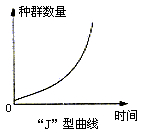
\includegraphics[width=8cm]{J.jpg}
			\end{center}
			
			无论是微分方程的解法还是生物学的理论,皆非此处所关心的重点问题。我们所关注的问题是:真实世界中,种群数量的增长真的是由这样的连续函数所确定的吗?事实上并非如此,因为一方面种群个体的数量总是整数,不可能遍历一个区间;另一方面,种群个体的数量也并非无时无刻不在增加,也就是说那个增长率$b$不可能表现为一个瞬态的变化系数。这些问题的根源归结于:种群个体数量增长这样一个过程,本来就是一个离散的过程;因此,出生率$b$也最多只能是关于一段足够长的时间所计算出来的比率,不可能用于描述连续的变化过程。在现实情况下,我们对于种群个数的记录总是离散的,例如我们选择每一年记录一次种群的数量——这时$t$只能取整数年,相应的变化模型则应表述为
			\[
				\frac{\Delta N}{\Delta t}=Nb_y
			\]
			这里$\Delta t$恒为一年,而$b_y$则表示年出生率——我们仍然假设其是恒定的。微分模型被转化为离散模型(也就是差分模型),种群的数量最终也并不会表现为指数函数了——它只会是一系列看起来呈指数增长的离散数据点而已。(如果结合$N(t)$的意义要求该函数在每一个时刻都应有值,那么函数图像就会是一个所谓分段函数的形态。)
			
			从这个例子我们可以得到什么?尽管在大多数自然科学问题中我们总是不自觉的使用那些在区间上任何实数点处都有值的函数(也就是一般人所理解的“连续函数”)来作为实际问题的数学模型,但我们所面对的现实世界却往往是离散的、不便于处理的。这一方面源于某些自然规律或实际问题本身就是以离散的变化而呈现出来(例如种群个体的出生与死亡,银行存款的利息生成,乃至量子论的相关结果),另一方面也出自于观测这一行为本身的有限性——我们不可能观测到无限个数据点,人眼有最小的视觉分辨频率,电子设备也有采样的时间间隔。这一系列原因导致我们所最终接触到的世界总是以离散的形态呈现于我们的面前,尽管我们倾向于认为这些离散形态因其极小的时间间隔而可被毫无顾忌的用连续模型加以概括。连续的函数在许多时候都比离散的数据更易于理解和应用——前提是这种连续的规律足够简单并已经为人类认识研究的足够透彻,例如初等函数或一部分特殊函数。
			
			在数学理论的领域以内,我们可以说有许许多多不同的函数,且在上一节我们也认识到只有连续函数能够通过相对“稀疏”的点加以确定,其余函数则可任意的改变它们在那些奇异点处的取值而不受约束。但是,在实际科学问题中,我们却会发现:我们最终所拥有的只有{\bfseries 连续函数}——包括一部分只有少数间断点的“几乎”连续函数。为何如此?因为我们总是在观测、记录数据时作出这样一个假设:
			\begin{quote}\itshape
				观测和记录所得的数据,已经足以确定该函数的变化规律而没有过分的偏差。
			\end{quote}
		
			这不是与连续函数的性质十分类同吗?区别仅在于,我们的观测和记录总是有限的,因此即使是确定连续函数所要求的“所有有理点处函数值”我们也不可能全部获得。但总体而言,通过缩小观测间隔,我们可以保证观测结果的足够“充分”,接下来通过插值的方法所得的近似曲线之相对误差可以降到自然科学所容忍的范围以内。这“缩小观测间隔”的目的,也无非就是为了保证一件事情:
			\begin{quote}\itshape
				在任意给定的时间点周围足够近的时间范围内,总是存在已经观测到的数据点。
			\end{quote}
		
			这样,再利用连续函数的特性,我们便可以放心的认为:利用观测数据加上插值等连续化方法所得到的函数曲线,基本上能够反映被观测量、被研究问题的真实情况。换句话说,在自然科学的领域内,我们利用连续函数在连续点附近{\bfseries 相对平滑}这一特性,来弥补观测有限这一问题,以降低其所造成的误差,保证科学规律最大的真实性。这就是连续函数在一般自然科学问题(特别是各种连续现象)中的重要意义与价值。
			
			而对于前面所言的那些离散模型问题(如生物种群数量),用连续函数来表征的意义在于将问题简单化,毕竟在较为简单的情形下微分方程比差分方程易于解决。再者,我们又何尝不能说生物种群在某一刻的数量是个小数呢?怀胎十月,我们不妨认为每过一个月这世界上就多了0.1个人,直到孩子诞生,人数达到1为止。所以,关于离散模型,我们也可以说是观测或记录上的间断所导致的,而连续函数的引入正是为了填补上那些没有数据点处的规律。
			
			当然,我们也得说,这里有很多例外。当我们的观测已经被约束局限于某些固定的特殊点,或待研究的现象表现为某种瞬时突变,连续函数的这种局域特性反而会显得多余,甚至会引发错误的结论。这时我们所应用的数学模型,又会有所改易。这些内容,在具体的学科领域之内,会有更加详细的讨论。
		}
	
		\subsection{概念延伸:稠密集确定连续函数}{
			前面我们一直在喋喋不休地重复“所有有理点确定连续函数”,这“所有的有理点”难道真的有什么特殊之处?其实,选取这一系列点为代表,有理数本身的诸多性质(比如可以表示为$p/q$)倒并没有发挥什么作用,唯一的要点在于:
			\begin{quote}\itshape
				任何一个实数的任意小邻域内都有有理数。
			\end{quote}
			正是这一条性质使得我们最终得以确认连续函数只需要有理点就可以完全确定。事实上,不限于有理数集,只要任何一个数集满足这样的性质,我们都可以证明函数在这个数集上的取值就能唯一的确定一个连续函数。因此,我们给出这样一个定义:
			\begin{quote}\itshape
				定义:设数集$A\subset B$,若任给$x\in B$及任意小的$\delta>0$,总存在$x'\in A$满足$\mid x'-x\mid<\delta$,则我们称$A$是$B$的一个{\bfseries 稠密子集},或称$A$在$B$中{\bfseries 稠密}。如果这里取$B=\mathbb{R}$,我们也常直称$A$是一个{\bfseries 稠密集}。
			\end{quote}
			于是,我们起初所讨论的那一个命题可以进一步拓展为:
			\begin{quote}\itshape
				连续函数在整个实轴上的取值,可以唯一地由其在一个稠密集上的取值所决定。
			\end{quote}
			稠密集决定一个连续函数。这正是连续函数的神奇之处:部分决定整体。当然我们也得承认,这不是一种魔术,而是因为连续这两个字已经给连续函数施加了非常强的约束,这种约束使得整个实数集显得“多余”了。
			
			关于稠密集,我们还可以有更多的思考。例如,有理数集显然是一个稠密集,那么在有理数集中移出有限多个有理数之后,所得到的数集还是稠密的吗?显然还是。(证明或理解,交由读者自己完成。)那么我们忍不住要问,实数集最小的稠密集是什么呢?也就是说,是否存在一个稠密集$S$是其他所有稠密集的子集呢?若是有这样的一个数集,我们就可以只靠某一函数在$S$上的取值来“最经济”地决定一个连续函数了。关于这个问题,我所能给出的结论是:空想是徒劳的,因为没有这样的“最小稠密集”——既然我们已经确认任意稠密集去掉有限个点仍然稠密,那么如果真有这样一个最小稠密集$S$,给它去掉若干个点又如何呢?这必然与其最小性矛盾。这些内容,读者若感到有很强的兴趣,欢迎自学点集拓扑理论的相关内容;点集拓扑算是数学理论的柱石之一,然而相关知识对于自然科学的意义却比较寥寥,因此在这里就不再多费口舌了。(这里有Matrix 67上的几个比较简单而有趣的稠密集问题:\href{http://www.matrix67.com/blog/archives/1480}{\underline {再谈稠密性:令人吃惊的稠密集及其交集}})
			
		}
	}
	\newpage
	\section{何谓“有理”分析:数学分析的知识结构}{
		以上我们讨论了连续函数的特殊价值。现在我们仍然从大家都有了解过的《高等数学》课本之中,再举出几个例子来——而它们并不是连续函数。
		\begin{itemize}
			\item Dirichlet函数:$D(x)=\begin{cases}
				1 &,x\in \mathbb{Q}\\
				0 &,x\notin \mathbb{Q}
			\end{cases} $
			\item Riemann函数:$R(x)=\begin{cases}
				\dfrac{1}{q} &, x=\dfrac{p}{q}\in \mathbb{Q}~,(p,q)=1\\
				0   &, x\notin \mathbb{Q}
			\end{cases}$
			\item 符号函数:$sgn(x)=\begin{cases}
				1 &  ,x>0 \\
				0 &  ,x=0 \\
				-1 & ,x<0
			\end{cases}$
			\item 一个分段函数\footnote{这个函数也被称作“拓扑学家的正弦函数(曲线)”。}$f(x)=\begin{cases}
				\sin\dfrac{1}{x} & ,x\ne0 \\
				0 & , x=0
			\end{cases}$
			
		\end{itemize}
	
		前面两个函数可以说是高等数学乃至数学分析课程中各种“不存在”、“不是”问题的常客,唯一的例外可能是在可积性理论中要求你证明“Riemann函数是可积的”这样一个出人意料的结论;符号函数存在一个跳跃间断点(第一类),而最后一个分段函数以$0$为其振荡间断点(第二类),总之它们的性质都相对于一般的连续函数要奇异许多,也不便于处理。
		
		但是最重要的一点却在这里:这些函数,无一例外,几乎都是以反例的形象出现在课程当中,而未“再当大任”。在间断点的对应章节以外何尝再见到过所谓的振荡间断点?Dirichlet函数、Riemann函数和符号函数可曾有过什么实际的应用?皆没有。这些在后续课程中发挥重要作用的函数,在微积分的基础课程中则只是表现为差劲的反例,从这里我们便可以看到一个非常强的偏向:
		\begin{quote}\itshape
			所谓的“高等数学”归根结底就是“连续函数论”。
		\end{quote}
		
		学过工科的复变函数课程的读者可能会马上联想到另外一个说法:
		\begin{quote}\itshape
			所谓的“复变函数”归根结底就是“解析函数论”。
		\end{quote}
		
		这两者有非常高的相似性。高等数学课程的要求似乎是要求学生掌握利用微积分工具对“各类”函数进行研究,然而事实上我们在这门课程中从头到尾研究的都是连续或至多有几个寥落的间断点的函数而已!这是否是一种局限呢?这是出自于课程的安排不足,还是来自于古典微积分工具本身的缺陷,或是源于我们的实际需要确实仅止步于此呢?以下我们就来讨论这一系列的问题。
		\subsection{数学分析/高等数学的知识框架}{
			这里我们应当首先列出数学分析或高等数学课程的具体知识框架,以便于我们来具体分析。为了简便起见,我仅按照一个非常粗略的结构来概述它们。读者若已经非常熟悉这些内容,请跳过。
			\begin{itemize}
				\item 逻辑基础:实数理论({\slshape 高等数学无})
				\item 基本工具:极限理论【 数列和数列极限 | 函数极限 | 函数的连续性,初等函数的连续性 | 函数的阶,等价无穷小 | 函数的一致连续性({\slshape 高等数学可能无}) 】
				\item 一元微分学【 导数和微分 | 微分中值定理,不等式 | Taylor公式 | 函数性质与函数作图 】
				\item 一元积分学【 不定积分(原函数) | 定积分的定义(Riemann积分) | 可积性理论({\slshape 高等数学无}) | Newton-Leibniz公式(微积分学基本定理) | 广义积分,敛散性判别 | 微元法,积分应用({\slshape 数学分析讨论稍少}) 】
				\item 多元微分学 【 理论基础:$\mathbb{R}^n$空间,其上的拓扑({\slshape 高等数学几乎不讨论}) | 多元函数及其极限 | 偏导数与全微分,梯度 | 隐/反函数存在定理,求导公式({\slshape 高等数学可能无}) | 多元函数Taylor公式({\slshape 高等数学可能无}) | 有/无约束极值问题 】
				\item 高维空间上的积分学 【 重积分(二重、三重积分) | 含参积分,敛散性判别({\slshape 高等数学无}) | 线面积分 | Green公式,Gauss公式,Stokes公式 | 场论初步 】
				\item 常微分方程初步({\slshape 数学分析常无,单独开一门专业课}) 【 简易常微分方程(分离变量,齐次,常数变易法,可降阶) | 高阶线性微分方程(组) | 恰当方程与积分因子 | 各类换元法 】
				\item 无穷级数理论 【 数项级数的敛散性判别(正项级数,一般项级数) | 函数项级数的收敛域 | 函数项级数的一致收敛性,极限换序理论({\slshape 高等数学可能无,或讨论不深}) | 幂级数,收敛半径,函数的幂级数展开 | Fourier级数初步({\slshape 部分教材或课程可能无}) 】
				
			\end{itemize}
			
			越过这长长的一段提纲,我们需要注意到一点:这看似庞杂的内容,其实可以归结为两个{\bfseries 中心}——以古典微积分及相应工具(导数、积分、常微分方程、无穷级数)为{\bfseries 理论安排的中心},以连续函数为{\bfseries 研究对象的中心}。前者是显性的,而后者却是隐性的;我们能见到许多名为《解析函数论》的书,却还没有见到过所谓《连续函数论》的书,因为并不是连续函数——而是古典微积分理论赋予了高等数学或者数学分析课程以最大的意义。(在复变函数理论中则有所不同,解析函数本身具有的优良性质在很大程度上引领了早期复变函数理论的研究。)
			
			尽管如此,我们却仍然需要意识到连续函数在这两门课程之中的重要性。对于数学系学生而言,其重要性倒是可以稍微搁置一边,毕竟连续函数只是他们将来要研究的各类函数和数学对象之中普普通通、轻松易懂的一类罢了;但对于将要走上工程或研究岗位、与实际问题打交道的学生们来说,连续函数(从这里开始我总是用这个词指代连续函数或只有少量简短点的函数之总称)却将是他们最经常甚至是唯一有可能接触到的数学对象\footnote{我们可能还会考虑到有诸如广义函数等等之类更多的东西,这里只能说是一种粗浅的表述吧。}——要和它们打一辈子的交道。这件事情从古典微积分诞生的数百年来,似乎都还没有发生过太大的变化——这反映了连续函数与实际问题之间非常特殊的一种联系。这是严谨、“完美”的理论在现实世界中一个最令人感到亲切的投影。
		}
		\subsection{从稠密集到连续集,从《数学分析》到《实变函数论》}{
			不知道读者是否对实数系理论有所了解?如果读者还完全没有接触过这一内容,不妨抽空读一读本博客中的两篇诙谐有趣的概述\href{https://www.cnblogs.com/xjtu-blacksmith/p/7616948.html}{\underline{实数系与实数定理(上)}}与\\\href{http://www.cnblogs.com/xjtu-blacksmith/p/7625717.html}{\underline{实数系与实数定理(下)}}。下面的内容都由实数理论的相关内容说起。
			
			我们知道,数学分析或高等数学所研究的对象,是“{\slshape 实数系上的函数}”;然而前面种种分析叙述已经表明,唯有连续函数是这两门课程的主线,对于工科生而言连续函数甚至是他们唯一熟悉的东西。一方面,我们已经讲清,在实际的工程、科学技术问题中,的确只有连续函数是最为适合的研究对象和理论依据;另一方面,我们也应当认识到,在数学分析或高等数学课程中所使用的古典微积分工具,本身就是出自于当时的数学家们对连续函数的研究、归纳与把握。
			
			就以古典的Riemann积分为例。齐民友先生的《重温微积分》一书中有一节标题为“{\slshape 这样评价Riemann公正吗}?”讨论的是Riemann积分的缺陷与不足究竟应当怎样看待。在现代数学家们看来,Riemann积分是非常粗糙的,法国的著名数学家Dieudonne在他的《现代分析基础》一书之中甚至完全没有涉及Riemann积分,原因是:
			\begin{quote}\itshape
				如果不是它的带有权威的名字,它老早就该没落下去了……现今这一“理论”的重要性在测度与积分的一般理论中,最多不过是一普通的有趣的练习……长久以后必将失去它的历史重要性。
			\end{quote}
			
			在此我们倒不必探讨Dieudonne先生的这个预言是否得到应验,反正到现在为止国内大部分数学系学生分析课本上的积分理论也还没有直接换成一般的测度积分理论。前沿数学家们持这样观点的原因在于,由Riemann最终概括总结的这套古典微积分理论,是出自于几百年前(Newton与Leibniz的时代)就基本成形的对连续函数和实际物理问题的研究。它虽然易于理解但缺乏一般性,完全可以充作现代分析理论下一个非常不起眼的特例来看待。这里我们是不是该惊呼数学家和其他自然科学工作者之间的巨大差异呢?
			
			数学史上有许多非常为人熟知的故事:所谓“函数”定义的\href{http://www.math168.com/sxsh/888.htm}{\underline{变迁}}(John Bernoulli, Euler, Cauchy, Fourier, Dirichlet, 一直到近现代的数学家们);分析学家关于收敛性(主要是级数收敛性)漫长的\href{https://wenku.baidu.com/view/8cbeadd376eeaeaad1f33046.html?sxts=1530453114865}{\underline{探索过程}};分析学的算术化(实数理论的建立)……从这一系列的故事中我们可以发现关键的一个线索:数学家从直观认识走向严谨理论经历了漫长的历史阶段,而这所谓的“直观认识”则正是今天的连续函数。没有人会在Newton或者Euler所在的时代提出所谓“处处不连续函数”或者“无穷多个间断点”——在他们看来,函数本来就应当是连续的,是一条曲线,是“随手画出来的”。从历史发展的角度来说,如果不是出现了某些危机(例如看似连续Fourier级数收敛于存在间断点的函数),我们完全可以把古典微积分的应用范围乃至数学研究的范围局限于连续函数类之中——就像最终是三次方程而不是二次方程推动了虚数和复数理论的发展。然而,一旦走出这和谐美好、符合直观的“温室”,数学家们似乎就再也没法走回来了,哪怕有许多的指责与质疑,因为在连续函数之外我们确实看到了许多更加丰富的内容,就像进入看似玄虚的复数域却给数学理论与科学技术领域带来了极大的方便。
			
			关于数学分析,我们要说的最重要的一点是什么呢?也许不仅仅是连续函数的问题了,而应当归结到实数系的性质上去:
			\begin{quote}\itshape
				古典微积分所研究的一切内容,几乎都仅限于实数系的数域性质、有序性质和阿基米德性质(即无界性质),而很少真正利用实数系独有的连续性。换句话说,我们完全可以仅在有理数集上建立一套微积分体系——只要我们稍稍修改相关定义即可。
			\end{quote}
			
			那么我们为什么还要将研究的范围扩张至实域呢?原因无非是:实数域是我们所认为真实存在的“数”之总和(可以参见\href{http://www.cnblogs.com/xjtu-blacksmith/p/7625717.html}{\underline{实数系与实数定理(下)}}的最后一节内容),因而有必要将其统一囊括起来,哪怕有理数之外的无理数在实际研究问题之中并不真正比有理数特殊多少,更何况我们应当指出我们所观测到和记录到的一切数据{\slshape 本质上}都是有理数。这是对于面向实际问题的学生们特别重要的一点,他们不必拘束于繁杂严谨的数学框架之下,而应当将更多的精力放在对于实际问题的研究与把握之上。理论的严谨与成体系与应用上的简洁方便总是存在着一点矛盾,这是有待于我们去解决的问题。
			
			由于有理数集不完备,我们当然可以找到无数个收敛于无理数的有理数列,这确实是理论上的空缺,需要由更加深刻完备的理论加以补充;但是,对于应用者而言,他完全可以不必理会这样的数列,如果他限定数列收敛于一个有理数或某个无理数的有理近似(如小数点后若干位)而已,那么这一类数列对他而言便没有任何研究的价值,诸如此类。我在这里想说的是,我们既要看到理论是如何一层一层完备严谨起来的,也要认识到在自己将来所要面临的领域与问题之中哪些东西是多余的、是不必考虑的。
			
			那么,在哪里我们真正的要让实数集的连续性派上用场呢?那就是数学系的实变函数课程了。本来在这里还可以接下去讨论许多有趣的内容,但写到这里我突觉如此将有破坏文章主旨之嫌,因此这些内容不妨留到以后有空时再专辟一章来叙述。读者切不要秉持流行的偏见,把实变函数论所研究的内容一并视为现实世界中不存在的反例、怪物;我想在这里引用齐民友老先生在《重温微积分》第四章中的一段评述:
			\begin{quote}\itshape
				反例的重要性在于它揭露了无法回避的矛盾。
			\end{quote}
			
			无论数学家与自然科学工作者各自怎样看待这些课程、知识、内容,他们一定都会赞同一个结论:我们的知识与科学,总是需要不断的前进与提高,而这是每一个人的责任。
			
		}
	
	}
	
\end{document}